 \chapter{Generierung von Landschaftsbildern}\label{chp:bildgenerierung} % 10 Seiten
 \glsresetall

 Der erste Teil des vorliegenden Projektes beschäftigt sich mit dem Generieren
 von neuen Landschaftsbildern aus Zufallsvektoren. Dazu wird das Konzept der in
 \cref{GANs} beschriebenen \gls{acr-GAN} verwendet.
 
 \section{Modelle}% Joshua

 Wie in \cref{GANs} beschreiben, gibt es im Bereich der \gls{acr-GAN}s
 zahlreiche Varianten und Anpassungen, die versuchen, verschiedene Schwachstellen
 des Konzeptes auszugleichen. Um dieser Vielzahl von Möglichkeiten zu begegnen,
 wurden in diesem Projekt zwei weit verbreitete \cite{kurach2018gan}
 GAN-Architekturen umgesetzt, das \emph{\gls{acr-DCGAN}}
 \cite{radford2015unsupervised} zusammen mit dessen Erweiterung zum
 \emph{\gls{acr-SNDCGAN}} \cite{miyato2018spectral}, sowie das
 \emph{\gls{acr-WGAN}} \cite{arjovsky2017wasserstein}. 

\subsection{SNDCGAN}\label{subsec:mod:sndc} % Joshua
\label{sub:sndcgan}

Das erste im Projekt umgesetzte \gls{acr-GAN} Modell, ist das \gls{acr-SNDCGAN},
welches
in dieser Form aus dem Übersichts-Paper
\citetitle{kurach2018gan} von \citeauthor{kurach2018gan} \cite{kurach2018gan}
übernommen ist. Dieses Modell ist eine Erweiterung des im Paper
\citetitle{radford2015unsupervised} von \citeauthor{radford2015unsupervised}
\cite{radford2015unsupervised} vorgestellten \gls{acr-DCGAN}s um die Änderungen
des SN-GANs aus \citetitle{miyato2018spectral} von
\citeauthor{miyato2018spectral} \cite{miyato2018spectral}. Dies wird im Projekt
durch die Standard-Kostenfunktion des ursprünglichen \gls{acr-GAN}s
\cite{goodfellow2014generative}, sowie einem leicht angepassten
Trainingsprozedere ergänzt.

\paragraph{\gls{acr-DCGAN}} Die Idee des \gls{acr-DCGAN} von
\citeauthor{radford2015unsupervised} \cite{radford2015unsupervised} ist es die
ursprünglich \cite[vgl.][]{goodfellow2014generative} auf vollständig verbundenen
Schichten (\emph{fully connected} bzw. \emph{Multilayer Perceptron (MLP)})
basierende \gls{acr-GAN}-Architektur mit dem speziell für Bildverarbeitung
attraktiven \gls{acr-CNN} zu verbinden \cite{radford2015unsupervised}.
Dabei nutzt das \gls{acr-DCGAN} bestimmte (zu der Zeit) aktuelle Entwicklungen
der \gls{acr-CNN}s \cite[vgl.][S. 3]{radford2015unsupervised}: Auf
deterministische Pooling-Funktionen wird zugunsten von \emph{strided
Convolutions} (d.\,h. Convolutions bei denen der Kernel um mehr als eins pro
Schritt bewegt wird) verzichtet; es werden bewusst gar keine (versteckten)
vollständig verbunden Schichten verwendet; es wird Batch-Normalisierung (d.\,h.
das Normalisieren der Eingabe zu einem Mittelwert von null und einer Varianz von
eins) auf die meisten Schichten angewandt und es wird \emph{ReLU} als
Aktivierungsfunktion (bis auf die Ausgabeschicht, die tanh verwendet) für den
Generator bzw. \emph{Leaky ReLU} für den Discriminator verwendet.
\gls{acr-DCGAN} beansprucht für sich, vor allem durch diese Änderungen, das
Training im Vergleich zu anderen Ansätzen stabilisieren zu können \cite{radford2015unsupervised}.

\paragraph{\gls{acr-SNDCGAN}} Das Paper \citetitle{miyato2018spectral}
\cite{miyato2018spectral} führt hauptsächlich eine neue
Gewichtsnormalisierungs-Technik ein, die aber für die
Pro\-jekt-Imp\-le\-men\-tier\-ung hier nicht relevant ist. Allerdings führt das
Paper auch einige geringe Änderungen an der Architektur des \gls{acr-DCGAN}s
ein, die für die Architektur des Projektes übernommen wurde. Dazu gehört
hauptsächlich die Nutzung eines acht-schichtigen Discriminators \cite{kurach2018gan}. Dies wird von \citeauthor{kurach2018gan} \cite{kurach2018gan}
als \gls{acr-SNDCGAN} bezeichnet. Das \gls{acr-SNDCGAN} beansprucht für sich vor
allem diversere Datenpunkte zu erzeugen (d.\,h. den Zufall des Zufallsvektors
besser umzusetzen) und einen besseren \gls{acr-IS} (eine Metrik für das
Beurteilen von \gls{acr-GAN}s) zu erreichen \cite{miyato2018spectral}.

\paragraph{Architektur} Die Architektur des \gls{acr-SNDCGAN}s, so wie es in
diesem Projekt umgesetzt wird, stammt aus \citetitle{kurach2018gan}
\cite{kurach2018gan} und ist in \cref{tab:sndcgan} beschrieben. Dabei sieht man,
wie im Discriminator das Bild über Convolutions schrittweise verkleinert wird,
gleichzeitig aber mehr Kanäle, d.\,h. mehr Informationen über das Bild
hinzukommen. Der Generator andererseits verwendet
Deconvolutions\footnote{Korrekterweise handelt es sich hierbei eigentlich um
\emph{Transposed Convolutions} auch \emph{Fractionally Strided Convolutions}
genannt, nicht um Deconvolutions (d.\,h. die mathematische Umkehrung der
Convolution) im engeren Sinne; allerdings wird in der Literatur häufig dennoch
von Convolutions gesprochen, was hier übernommen wurde \cites[vgl.][S.
20]{dumoulin2016guide}[vgl.][S. 4]{radford2015unsupervised}.} um aus dem
eindimensionalen Zufallsvektor schrittweise ein Farbbild zu erzeugen. Der
Bildgenerierungsprozess des Generators ist auch auch in \cref{img:sndcgan}
graphisch dargestellt, hier wird aus einem Zufallsvektor der Größe $128$
schrittweise ein $64 \times 64$ Bild erzeugt.

\begin{table}[]
  \caption{SNDCGAN Architektur}
  \label{tab:sndcgan}
  \begin{center}
    \begin{minipage}{.5\linewidth}
      \caption{SNDCGAN Discriminator}
      \centering
        \begin{tabular}{lcl}
            \toprule
            Schicht & Kernel & Ausgabe\\
            \toprule
            Conv, lReLU & $[3,3,1]$ & $h \times w \times 64$\\
            \midrule
            Conv, lReLU & $[4,4,2]$ & $h/2 \times w/2 \times 128$\\
            \midrule
            Conv, lReLU & $[3,3,1]$ & $h/2 \times w/2 \times 128$\\
            \midrule
            Conv, lReLU & $[4,4,2]$ & $h/4 \times w/4 \times 256$\\
            \midrule
            Conv, lReLU & $[3,3,1]$ & $h/4 \times w/4 \times 256$\\
            \midrule
            Conv, lReLU & $[4,4,2]$ & $h/8 \times w/8 \times 512$\\
            \midrule
            Conv, lReLU & $[3,3,1]$ & $h/8 \times w/8 \times 512$\\
            \midrule
            Linear & - & $1$\\
            \bottomrule
        \end{tabular}
    \end{minipage}%
    \begin{minipage}{.5\linewidth}
      \centering
        \caption{SNDCGAN Generator}
        \begin{tabular}{lcl}
            \toprule
            Schicht & Kernel & Ausgabe\\
            \toprule
            $z$ & - & $128$\\
            \midrule
            Linear, BN, ReLU & - & $h/8 \times w/8 \times 512$\\
            \midrule
            Deconv, BN, ReLU & $[4,4,2]$ & $h/4 \times w/4 \times 256$\\
            \midrule
            Deconv, BN, ReLU & $[4,4,2]$ & $h/2 \times w/2 \times 128$\\
            \midrule
            Deconv, BN, ReLU & $[4,4,2]$ & $h \times w \times 64$\\
            \midrule
            Deconv, Tanh & $[3,3,1]$ & $h \times w \times 3$\\
            \bottomrule
        \end{tabular}
    \end{minipage} 
  \end{center}
  \begin{center}
    \bigskip
    \emph{Quelle:} Von \cite[S. 12]{kurach2018gan} übernommen.\\
    \emph{Legende:} Der Kernel ist beschrieben im Format $[\text{x\_Größe},
    \text{y\_Größe}, \text{Schrittweite}]$; $h$ und $w$ beschreiben die Höhe
    bzw. Breite des Eingabe-Bildes in Pixeln; damit beschreibt die Ausgabe
    $\text{Höhe} \times \text{Breite} \times \text{Kanäle}$, wobei das
    Eingabe-Bild als farbiges Bild drei Kanäle hat.
  \end{center}
\end{table}

\begin{figure}
  \caption{SNDCGAN Architektur des Generators}
  \label{img:sndcgan}
  \centering
  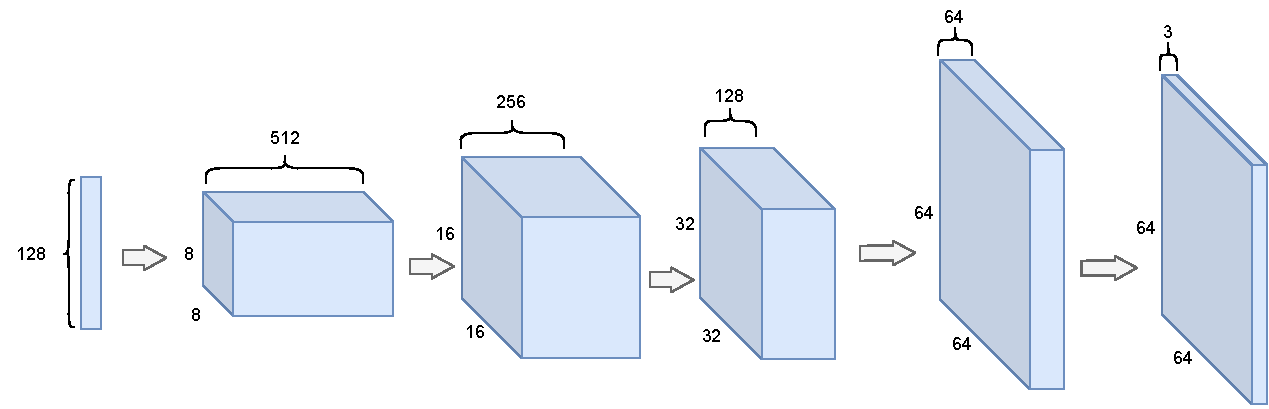
\includegraphics[width=\textwidth]{images/cnn3.pdf}
\end{figure}

\paragraph{Kostenfunktion} Als Kostenfunktion wird für die
Projekt-Implementierung entsprechend des \gls{acr-SNDCGAN} Papers die
ursprüngliche Standard-Kostenfunktion aus dem Paper von
\citeauthor{goodfellow2014generative} \cite{goodfellow2014generative} verwendet.
Diese ist gegeben als $V(D, G) = \mathbb{E}_{x \sim p_{\text{data}}(x)} [\log
D(x)] + \mathbb{E}_{z \sim p_{z}(z)} [\log (1-D(G(z)))]$. Dabei wird davon ausgegangen, dass der
Discriminator $D$ eine $1$ ausgibt, wenn er der Ansicht ist, dass das
eingegebene Bild sicher ein original Bild der Daten ist. Damit ist das Ziel des
Discriminators $V(D,G)$ zu maximieren, während der Generator die Funktion
minimieren möchte: $\min_{G} \max_{D} V(D,G)$. In der Praxis des Projektes wird,
ebenfalls dem \gls{acr-SNDCGAN} und \gls{acr-GAN} Papern folgend \cites{goodfellow2014generative}{miyato2018spectral}, statt der Minimierung
von $\log(1-D(G(z)))$, $\log D(G(z))$ maximiert, dies verringert das Problem von
verschwindenden Gradienten im frühen Training.

\paragraph{Training} Das Training der Projekt Implementierung folgt im
wesentlichen dem von \citeauthor{goodfellow2014generative}
\cite{goodfellow2014generative}. Der Generator und Discriminator werden jeweils
abwechselnd trainiert, wobei zuerst der Generator eine Batch von Beispiel-Daten
erzeugt, die anschließend vom Discriminator bewertet werden. Dies wird zuerst
für die Kosten des Generators verwendet und anschließend, zusammen mit einer
Bewertung von Originaldaten durch den Discriminator, für das Training des
Discriminators. Den Lernverfahren der einbezogenen Paper
\cite{radford2015unsupervised,miyato2018spectral,kurach2018gan} folgend,
verwendet die Implementierung des Projektes den Adam-Optimizer
\cite{kingma2014adam}.
 
 \subsection{Wasserstein-GAN} % Tim
 Das \gls{acr-WGAN} wurde 2017 in \citetitle{arjovsky2017wasserstein}
 \cite{arjovsky2017wasserstein} vorgestellt. Dabei verwendet dieses einen
 alternativen Weg um den Generator zu trainieren, welcher die Datenverteilung
 der gegebenen Trainingsdaten besser approximieren soll. Anstatt einen
 Discriminator zu verwenden, der Bilder in real oder nicht real kategorisiert,
 verwendet das \gls{acr-WGAN} einen einen \enquote{Critic}, welcher durch einen
 linearen Wert Bilder nach ihrem Realismus bewertet. 
 
 Für die Aufgabe Landschaftsbilder zu generieren wurde ebenfalls ein
 \gls{acr-WGAN} implementiert. Aufgrund fehlender Trainingsressourcen konnte
 diese Implementation jedoch nicht optimiert werden und liefert deutlich
 schlechtere Ergebnisse als die \gls{acr-SNDCGAN} Implementierung. Dennoch ist
 das \gls{acr-WGAN} eine interessante Möglichkeit ein Generator zu erschaffen.  
 
 \paragraph{Architektur} Die in diesem Projekt verwendete Architektur des
 \gls{acr-WGAN}s orientiert sich an der des \gls{acr-SNDCGAN}s, beschrieben in
 \cref{sub:sndcgan}. Allerdings wurden weniger Convolutions verwendet um
 Ressourcen zu sparen, da die Architektur noch nicht optimiert wurde. Der Critic
 verwendet ebenfalls Convolutions, und fügt diese am Ende zu einem linearen Output zusammen \cite{brownlee_how_2019-1}.
 Außerdem werden die Gewichte im Critic zwischen -0.01 und 0.01 beschränkt
 \cite{arjovsky2017wasserstein}. 
 
 \paragraph{Kostenfunktion} Das \gls{acr-WGAN} verwendet den Wasserstein-Loss,
 welcher versucht den Abstand zwischen realen und generierten Bildern zu
 maximieren. Dabei können die Kostenfunktionen nach \cite{brownlee_how_2019}
 folgendermaßen definiert werden:
 \begin{itemize}
 	\item Critic Loss = [Durchschnittlicher Critic Wert auf realen Bildern] –
 	[Durchschnittlicher Critic Wert auf generierten Bildern]
 	\item Generator Loss = -[Durchschnittlicher Critic Wert auf generierten
 	Bildern]
 \end{itemize}

\paragraph{Training} Einer der großen Vorteile des \gls{acr-WGAN}s ist, dass es
keinen Discriminator gibt, der dem Generator \enquote{davonläuft}. Ein besserer
Critic sorgt für bessere Ergebnisse \cite{arjovsky2017wasserstein}.
Deshalb wird beim Training der Critic mehr trainiert, als der Generator, in
diesem Fall fünf mal so oft. Zudem wird RMSProp statt Adam als Optimizer
verwendet \cite{arjovsky2017wasserstein}.
 
  \section{Implementierung} % Jonathan
  \label{sec:gen_impl}
 
 Der folgende Abschnitt thematisiert die Implementierung des zuvor beschriebenen
 SNDCGAN-Modells in Tensorflow bzw. Keras. Außerdem wird auch die Optimierung
 der Parameter der Netze behandelt.
 
 \subsection{Umsetzung in Tensorflow/Keras}\label{subsec:imp:sndc}
 
 Ein wichtiger Teil der Implementierung ist die Überführung der in
 Abschnitt~\ref{subsec:mod:sndc} vorgestellten Architektur des SNDCGANs in ein
 Tensorflow-Modell. Dafür wird das \glqq Sequential Model\grqq\ von
 Keras~\cite{keras:SequentialModel} verwendet. In dem Modell werden die
 benötigten Schichten des Generators und des Discriminators definiert. Beim
 Trainieren wird der Input sequenziell von einer Schicht zur nächsten
 durchgereicht und adaptiert, daher auch die Namensgebung.  
 
 Nachdem die Architektur des SNDCGANs zu Beginn des Projektes implementiert war,
 konnten erste Tests durchgeführt werden. Dabei war es ein großes Problem, dass
 der Fehler des Discriminators schnell auf null ging und damit der Generator
 keine Chance mehr hatte, irgendetwas zu lernen bzw. zu verbessern, da jeder
 Versuch als künstliches Bild enttarnt wurde und der Generator somit keine
 Erfolge mehr verbuchen konnte. Aus diesem Grund wurde die Architektur des
 Discriminators angepasst und Dropout eingeführt. Dadurch werden bei jedem
 Trainingsvorgang nur ein Teil der Neuronen trainiert und der Generator bekommt
 eine Chance, sich gegen den Discriminator durchzusetzen.
 
 Die komplette Implementierung der am Ende verwendeten Architektur beider
 Modelle ist im Anhang unter \autoref{lst:sndcGenerator} und
 \ref{lst:sndcDiscriminator} zu finden.
 
 Weiter wird für das Trainieren des SNDCGANs eine Trainingsschleife benötigt.
 Die in diesem Fall verwendete Schleife wurde zunächst aus \cite{raschka2019}
 übernommen und im Folgenden an die Bedürfnisse des Projektes angepasst. Um die
 Gradienten für ein anschließendes Gradientenabstiegsverfahren zu berechnen,
 werden GradientTapes von Tensorflow~\cite{tf:gradientape} eingesetzt. Diese
 speichern alle Operationen, die bei der Ausführung des zu trainierenden Netzes
 durchgeführt werden und können daraus dann die Gradienten
 berechnen~\cite{tf:autodiff}.
 
 Um die neuronalen Netze zu optimieren, wird der Adam Algorithmus eingesetzt.
 Dieser führt einen Gradientenabstieg durch und wird bereits von Tensorflow zur
 Verfügung gestellt~\cite{tf:adam}. Als Besonderheit bringt Adam u. a. eine über
 die Zeit abnehmende Lernrate mit~\cite{kingma2014}.
 
 Ein weiterer wichtiger Teil der Implementierung ist die Möglichkeit, das
 Training zu pausieren und später wieder an gleicher Stelle aufzunehmen. Dies
 war vor allem wichtig, da die Rechenkapazitäten für dieses Projekt sehr
 begrenzt waren, somit das Trainieren viel Zeit in Anspruch genommen hat und das
 Training dabei nicht an einem Stück durchgeführt werden konnte. Deshalb wurde
 implementiert, dass in regelmäßigen Abständen Checkpoints des Lernfortschritts
 gespeichert werden. Diese Umfassen neben den Modellen des Generators und
 Discriminators auch deren Optimizer. Dies ist wichtig, da wie zuvor erwähnt
 wurde, die Lernrate der Adam Optimizer über die Zeit abnimmt. Somit ist nur
 eine Fortsetzung des Trainings beim gleichen Stand möglich, wenn auch die
 bisher verwendeten Optimizer geladen werden. 
 
 Zunächst war geplant, dass diese Checkpoints dauerhaft gespeichert werden,
 damit die trainierten Netzwerke später ausgewertet und verwendet werden können.
 Bei Testläufen hat sich allerdings herausgestellt, dass jeder Checkpoint fast
 600 MB umfasst und dies sich dann über die ganzen Epochen zu einem großen
 Speicherverbrauch aufsummiert. Deshalb wurde zusätzlich eingeführt, dass die
 trainierten Modelle einzeln gespeichert werden und von den Checkpoints nur noch
 die letzten zwei erhalten bleiben. Dadurch konnte der Speicherplatz pro
 gespeicherter Epoche um zweidrittel reduziert werden.
 
 \subsection{Anpassung von Parametern} % Jonathan
 
 Eine große Herausforderung in diesem Projekt war die richtige Wahl der
 Parameter für das Training. Diese müssen so gewählt werden, dass das neuronale Netz möglichst gut
 initialisiert wird, um dann gute Ergebnisse zu produzieren. Dabei war das
 Hauptproblem die fehlende Rechenkapazität, um verschiedene Konfigurationen
 ausführlich auszutesten, anschließend mit einer wissenschaftlichen
 Herangehensweise zu vergleichen und daraus die besten Parameter abzuleiten. Aus
 diesem Grund mussten die Entscheidungen auf Basis weniger Versuche getroffen
 werden. Daher ist es mit Sicherheit möglich, anhand einer ausführlicheren
 Analyse besser passende Parameter zu finden.
 
 Im Folgenden werden die vier Variablen \emph{Droprate}, \emph{initiale
 Lernrate}, \emph{Bildermenge} und \emph{Auflösung der Bilder} genauer
 thematisiert.
 
 Wie im vorherigen Abschnitt~\ref{subsec:imp:sndc} bereits erwähnt wurde, war es
 zu Beginn des Projektes ein großes Problem, dass der Fehler des Discriminators
 nach kurzer Zeit auf null ging und damit einen Lernfortschritt des Generators
 unmöglich machte. Neben der Einführung des Dropouts, war auch die Anpassung der
 initialen Lernrate auf der Seite des Discriminators wie auch auf der des
 Generators eine wichtige Stellschraube. Während es bei der Droprate auf Basis
 eines Blogbeitrags~\cite{brownlee2019} relativ schnell möglich war, einen Wert
 von 50 \% festzulegen, mussten bei der Lernrate einige Testläufe absolviert
 werden. 
 
 Die zu Beginn gewählten Lernraten bewegten sich in der Größenordnung von E-3
 und mit ihnen trat das Verschwinden des Discriminator-Fehlers auf. Eine
 Vergrößerung der Lernrate wirkte sich deutlich negativ auf das Lernverhalten
 aus, da der Fehler des Discriminators noch schnell zu null ging. Als dritten
 Ansatz wurden unterschiedliche Lernraten für Generator und Discriminator
 getestet. Dabei wurde die des Generators im Bereich von E-3 deutlich größer
 gewählt als die des Discriminators mit E-4. Das Ziel war, den Generator
 schneller lernen zu lassen, als den Discriminator. Allerdings waren die
 Ergebnisse damit auch noch nicht zufriedenstellend. Erst ein Reduzieren beider
 Lernraten in den Bereich von E-4 hat für sichtbare Veränderungen bei den
 produzierten Beispielbildern gesorgt.
 
 Um den Trainingsprozess bei diesen Versuchen zu beschleunigen, wurde immer nur
 mit relativ wenig Bildern gelernt. Erst nachdem die ersten Erfolge durch eine
 bessere Wahl der initialen Lernrate sichtbar wurden, erhöhte sich die
 Bildermenge auf zunächst ca. 1500 Stück und später dann auf etwas mehr als
 7000, was auch eine weitere Verbesserung der Ergebnisse mit sich brachte.
 Allerdings beschränkten sich die Verbesserung auf sichtbare Änderungen in den
 abgebildeten Formen, die zunehmend komplexer wurden. Die erstellten Bilder
 hatten jedoch noch wenig Ähnlichkeit zu (schlecht aufgelösten)
 Landschaftsbildern.
 
 Die letzte Änderung, die anschließend zu zufriedenstellenden Ergebnissen
 geführt hat, war eine Vergrößerung der Auflösung. Das bis dahin mit einer
 Bilderauflösung von 128x72 Pixeln trainierte SNDCGAN wurde auf 256x144 Pixel
 vergrößert. Dies bedeutete zwar einen deutlich Anstieg der Rechenzeit,
 allerdings war damit in den Beispielbildern mehr Inhalt zu erkennen, den das
 GAN lernen konnte.
 
 \section{Evaluierung}\label{evalGen} Nachdem das Training des implementierten
  GANs erfolgreich abgeschlossen wurde, siehe \cref{fig:landschaftsbilder}, erfolgt die Evaluation der Ergebnisse.
  Dafür wurden zwei verschieden Methoden genutzt. Die Erste betrachtet den
  durchschnittlichen Loss des Generators und Discriminators, zu sehen in
  Abbildung \ref{fig:plot_losses_gen}.  Hier ist zu erkennen, dass zu Beginn
  Spitzen von großen Losses auftreten, diese sich aber im Verlauf zu späteren
  Epochen auspendeln und zu einem Minimum tendieren. Daraus kann gefolgert
  werden, dass die Netze ihre Aufgabe erfüllen, nämlich die Losse beider Netze
  zu minimieren. In den letzten hundert Epochen ist eine steigende Tendenz zu
  beobachten, die auf ein Overfitting zurückgeführt werden kann.
 
 \begin{figure}
 	\centering
 	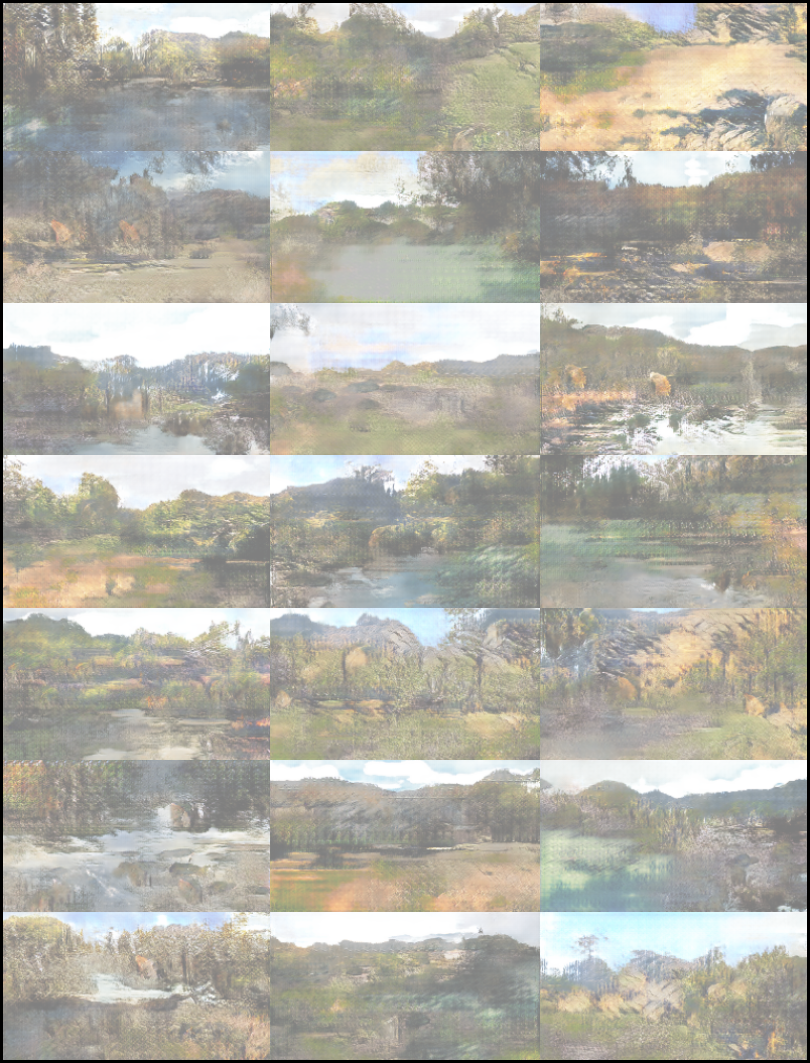
\includegraphics[width=\linewidth]{images/Landschaftsbilder}
 	\caption[Ergebnisse Generierte Landschaftsbilder]{Sammlung von 21 Bilder die durch das SNDCGAN produziert wurden.}
 	\label{fig:landschaftsbilder}
 \end{figure}
 
 
 \begin{figure}[t]
 	\centering
 	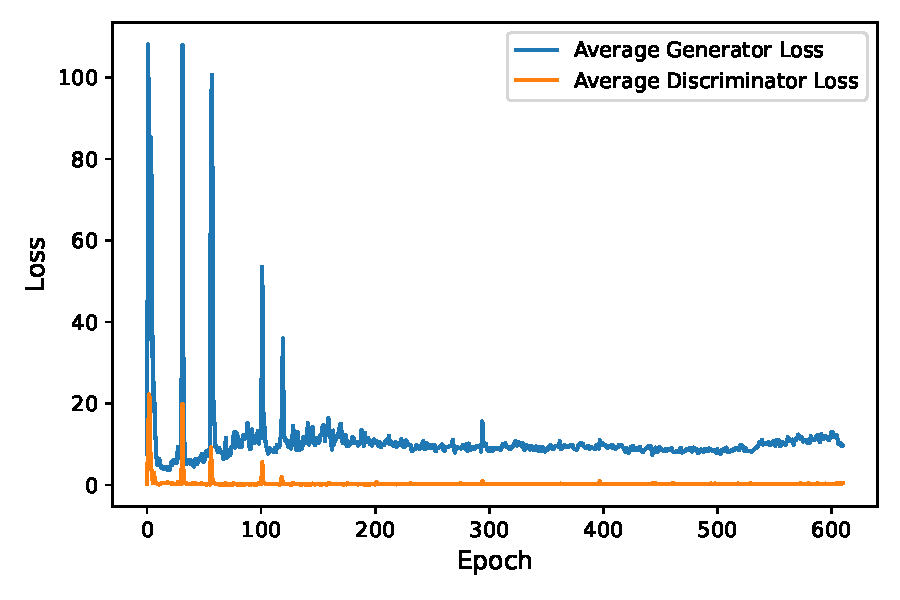
\includegraphics[width=0.7\linewidth]{images/plot_line_plot_losses_gen}
 	\caption[Losses des generirenden GANs]{Der Loss über alle Epochen des GANs , welches für das generieren von Landschaftsbilder genutzt wurde.}
 	\label{fig:plot_losses_gen}
 \end{figure}
 
 Die zweite Methode ist das Berechnen der \acrfull{acr-FID}. Diese bestimmt die
 Ähnlichkeit der echten und der generierten Bilder \cite{heusel_gans_2017}. Dies
 wird über die Fr\'echet Distanz gemacht, welche die Gaußglocken der
 Verteilungen beider Domänen vergleicht. Die Gaußglocke wird über den Mittelwert
 $m$ und die Kovarianz $C$ festgelegt. 
 
 \[d^2((m,C),(m_w,C_w)) =  \|m-m_w\|^2_2 + trace(C+ C_w - 2(CC_w)^{\frac{1}{2}})
 \]
 
 Die in dieser Arbeit umgesetzte Implementierung von \gls{acr-FID} geht über
 alle gespeicherten Modelle des Generators (hier jede fünfte Epoche). Anhand dieser
 werden  
 mittels über alle Epochen gleichbleibenden Zufallsvektoren Bilder generiert.
 Diese Bilder werden nun mit einer zufälligen aber festen Auswahl an echten
 Bilder verglichen, in dem alle Bilder durch den besten Discriminator bewertet
 werden. Beim Discriminator müssen die letzten beiden Schichten entfernt werden
 und durch eine Pooling-Schicht mit anschließendem Abflachen ersetzt werden,
 damit die Berechnung der Mittelwerte und Kovarianzen durchgeführt werden kann. 
 
 Die Auswertung des genutzten Modells unter Verwendung des Discriminators mit
 geringsten Loss ist in Abbildung \ref{fig:plot_fids_gen} sichtbar. Über die
 Approximation ist klar zu erkennen, dass der Wert im Laufe der Zeit fallend
 ist, was eine Annäherung der generierten Bilder zu den echten Bilder
 widerspiegelt. Genau diese Eigenschaft ist bei der Generierung mittels GANs
 gewünscht.
 
 \begin{figure}
 	\centering
 	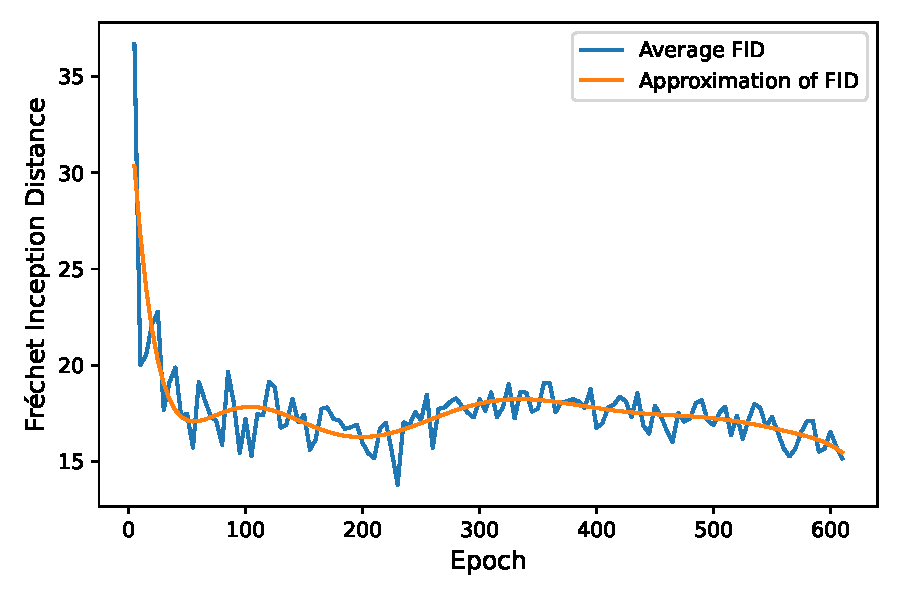
\includegraphics[width=0.7\linewidth]{images/plot_line_plot_fids_gen}
 	\caption[FID des generierdene GANs]{FID über alle Epochen mit dem Discriminator aus Epoche 535}
 	\label{fig:plot_fids_gen}
 \end{figure}
 
 Das Fazit aus den beiden Evaluierungsmethoden ist, dass das in dieser Arbeit
 implementierte und trainierte GAN die Aufgabe des Generierens von
 Landschaftsbilder gut umgesetzt hat. Die Losses des gesamten Netzes pendeln
 sich auf feste Werte ein, bei denen es sich um das Minimum handelt. Sowie die
 Ergebnisse der \gls{acr-FID} zeigen, dass die generierten Bilder relativ ähnlich
 zu echten Bilder sind, wodurch die generierten Bilder für den Menschen wie
 echte Landschaftsbilder wirken.
 %TODO: Bilder vergleich zeigen?
 
 